% % !TeX root = ../thuthesis-example.tex


\chapter{栈}
线性表是一个非常“开放的”数据结构,您可以读、写、插入和删除线性表上的任何一个数据单元。但在实际的计算模型中,并不是所有的数据结构都允许您这样做。
通过对允许访问的数据进行限制,我们可以过滤掉多余的信息,简化模型的复杂程度,从而更快更好地解决问题。

\textbf{栈}(stack)、\textbf{队列}(queue)以及\textbf{双端队列}(deque)就是典型的“访问受限制”的数据结构,它们的实现都是以线性表作为基础的;如果说线性表是“容器”,那么栈和队列这些结构更接近于“接口”,在C++ STL中称它们为容器\textbf{适配器}(adapter)。另一种经典的限制访问的数据结构是\textbf{优先队列}(priority queue),它需要以树作为基础,因此放到较后的章节讨论。
栈和队列限制了用户访问元素的范围,这使得它们能够防止用户做出对进程、系统、计算机或网络有害的“非法”行为,在《操作系统》和《网络原理》中都能看到它们的应用。
本章将首先讨论栈及其应用。

\section{栈的性质}

\subsection{栈的定义}
\label{sta:栈的定义}
\textbf{栈}(stack)是一种特殊的线性表。对于栈$S[0$:$n]$,它的插入、访问(因为只能读一个元素,不存在“查找”)、删除操作均只能对\textbf{栈顶}元素(top或peek,即栈的最后一个元素)$S[n-1]$进行。如图\ref{fig:sta1}所示,当栈顶为$x$时,三种操作都只能在$x$处进行。红色标出了操作之后的新栈顶,蓝色标出了操作之后的不可访问区域。

\begin{figure}
  \centering
  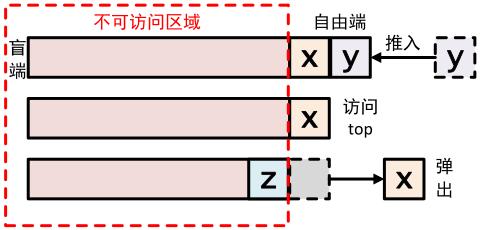
\includegraphics[width=0.7\linewidth]{figures/sta1.pdf}
  \caption{栈的推入、访问、弹出}
  \label{fig:sta1}
\end{figure}

\begin{enumerate}
    \item 栈的插入就是在$S[n-1]$后面插入新的元素(称为\textit{入栈}或\textit{推入},push)。
    \item 栈的访问就是取$S[n-1]$。
    \item 栈的删除就是将$S[n-1]$从栈中删除(称为\textit{出栈}或\textit{弹出},pop)。
\end{enumerate}

由于弹出后的元素往往另有他用,出栈操作会将被删除的栈顶元素返回。

\begin{lstlisting}
template <typename T>
class AbstractStack : public DataStructure<T> {
public:
    virtual void push(const T& e) = 0;
    virtual T pop() = 0;
    virtual T& top() = 0;
};
\end{lstlisting}

\subsection{栈的结构}
\label{stack:栈的实现}
由于栈实质上是对线性表的访问权限作出限定,所以很容易在线性表的基础上建立栈。以向量(顺序表)实现的栈称为顺序栈,以列表(链表)实现的栈称为链栈。您很容易自己实现一个栈,并使用\textit{StackTest.cpp}进行测试。

\begin{lstlisting}
template <typename T, typename Linear = Vector<T>>
    requires std::is_base_of_v<AbstractLinearList<T, typename Linear::position_type>, Linear>
class Stack : public AbstractStack<T> {
    Linear L;
public:
    constexpr static bool is_vector = std::is_base_of_v<AbstractVector<T>, Linear>;
    void push(const T& e) override {
        if constexpr (is_vector) {
            L.push_back(e);
        } else {
            L.push_front(e);
        }
    }
    T pop() override {
        if constexpr (is_vector) {
            return L.pop_back();
        } else {
            return L.pop_front();
        }
    }
    T& top() override {
        if constexpr (is_vector) {
            return L.back();
        } else {
            return L.front();
        }
    }
    size_t size() const override { return L.size(); }
};

\end{lstlisting}

这里需要注意的是,如果以向量(常规方式)实现栈,则我们总是使用末尾元素代表栈顶,就像在上一节所定义的那样。向量在头部做插入和删除操作的效率非常低,所以向量只能以尾部作为栈顶。但如果以单向列表实现栈,末尾元素变得不可访问,所以应当反过来以起始元素代表栈顶。双向列表因为是对称的,所以在末尾或起始都可以作为栈顶。

显然无论是顺序栈还是链栈,取顶的时间复杂度是$O(1)$,入栈和出栈的时间复杂度在分摊意义下也是$O(1)$。根据上一章的介绍您可以知道,用列表实现的栈,时间效率和空间效率都不如向量,但稳定性稍好。
在绝大多数应用场景下,使用向量实现栈都比使用列表实现栈更优,很少会出现使用链栈的场景。

\subsection{后入先出}

因为栈只能从尾部进行操作的特性,栈可以被写作$[ S_0, S_1, S_2, ..., S_{n-1} \rangle$的形式,左侧的中括号表示不可操作的一端(\textbf{盲端}),右侧的尖括号表示可操作的一端(\textbf{自由端})。更常见的一种表示方法是把它竖过来:

\begin{figure}
  \centering
  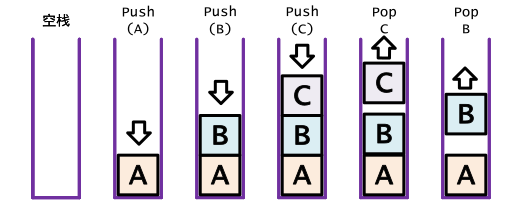
\includegraphics[width=0.8\linewidth]{figures/sta2.pdf}
  \caption{栈的桶式表示}
  \label{fig:sta2}
\end{figure}

如图\ref{fig:sta2}所示,可以把栈想成一个桶,盲端是桶的底部,自由端(栈顶)是桶中最上面的物品。于是,\lstinline{push}操作就是往桶里放东西,后放的东西总是放在先放的东西的上面,像上图中,B放在A上面,C放在B上面。而要取东西(\lstinline{pop})的时候,每次只能取桶里最上面的东西,也就是栈顶元素。在上图里,为了把B取出来,必须先把B上面的C取出来。

就像列表相关问题经常用链式图帮助思考一样,处理和分析栈的相关问题经常要用到上面这种桶式图。
从上图中不难发现,栈的最重要的性质是:\textit{先入栈的元素后出栈,后入栈的元素先出栈},简称为“\textbf{后入先出}”(\textbf{LIFO}, Last In First Out)。生活中有不少LIFO的例子,比如,桌子上一大摞书需要先搬开上面的才能拿下面的。这些现象被抽象化到计算机中处理就对应栈这种数据结构。严格来说,栈也应该采用LIFO进行定义,只要能够实现LIFO功能的数据结构都可以认为是栈,而不需要限制在\ref{sta:栈的定义}节中这种带盲端和自由端的线性表。不过由于这种单端自由的线性表实现非常简单,通常默认栈是用这种方法实现的。在《队列》和《优先队列》章中您将看到其他适配器结构会有多种不同的实现方法。

和栈相关的题目,通常有两个方向。

\begin{enumerate}
    \item 考察对栈性质(也就是LIFO)的理解。
    \item 在访问受限的情况下设计算法。
\end{enumerate}

在下面的几节,将介绍栈的几个应用以加深您对栈性质的理解。这些应用本身也是重要的考点,栈的大多数题目都出自这些应用。

\section{出栈序列}

\subsection{出栈序列的定义}

\textbf{出栈序列}(又称\textbf{栈混洗序列})是关于栈的一个重点问题。下面首先给出出栈序列的定义。

给定一个序列$A=(a_1,a_2,\dots,a_n)$,如果对于序列$B=(b_1,b_2,\dots,b_n)$,
存在对空栈$S$的入、出栈操作各$n$次的操作序列$O=(o_1,o_2,\dots,o_{2n})$,
使得当序列$O$中的入栈操作为依次将$a_1,a_2,\dots,a_n$入栈时,
序列$O$中的出栈操作出栈的元素恰好依次为$b_1,b_2,\dots,b_n$,
则称序列$B$为序列$A$的一个\textbf{出栈序列}。

操作序列中的每个元素是\lstinline{push}或者\lstinline{pop},为简化叙述,本书将使用$\lor$和$\land$分别表示它们。如果您用桶式图想象栈的形象,那么这两个符号是直观的。

一个显而易见的结论是:\textit{出栈序列是全排列的子集}。
以入栈序列为$(1,2,3)$为例,则$(3,2,1)$是它的一个出栈序列,对应的操作序列为$\lor\lor\lor\land\land\land$。您可以自己验证,$(2,3,1)$、$(2,1,3)$、$(1,3,2)$以及$(1,2,3)$自身,都是它的一个出栈序列;而$(3,1,2)$则无法成为一个出栈序列。

事实上,如果入栈序列是$(1,2,\dots,n)$,则$B=(b_1,b_2,\dots,b_n)$是出栈序列,当且仅当不存在“312”模式。即:不存在$i<j<k$,使得$b_j<b_k<b_i$。\textit{这个命题您可以在阅读了出栈序列的相关知识后自己证明。}

根据出栈序列的定义,可以立刻得到,在给定$A$的情况下,从$O$到$B$是一个满射。
那就自然地会引发猜想,从$O$到$B$也应该是一个单射。
这个问题可以用递归法分析,具体证明过程您可以自己补全。
设$O=(o_1,o_2,\dots,o_{2n})$中的最后一个$\lor$是$o_j$,则下一个操作$o_{j+1}$一定是$\land$,且$o_j$入栈的和$o_{j+1}$出栈的元素都是$a_n$。
那么,将$o_j$、$o_{j+1}$和$a_n$删除就递归到了$n-1$的情形。递归边界$n=1$结论显然。
这样,每个出栈序列就唯一对应了一个操作序列。

\subsection{出栈序列的计数}

从上一小节的分析可知,给定入栈序列的情况下,出栈序列的数量等于操作序列的数量,而操作序列$O=(o_1,o_2,\dots,o_{2n})$的数量和入栈序列的内容无关,只和入栈序列的长度$n$相关。

在这一小节中,先设长度为$2n$的操作序列$O$的数量是$f(n)$。
为了求解这个函数,需要确定操作序列$O$需要满足的条件。

\begin{enumerate}
    \item 包括$n$个$\lor$和$n$个$\land$。
    \item 对于操作序列的任意一个\textit{前缀},前缀中$\lor$的数量一定\textit{不小于}$\land$的数量。否则,在这个前缀的操作结束之后,栈的规模会变成负数,这是不可能的。
\end{enumerate}

容易验证满足上述两个条件的序列,也一定是合法的、可以生成对应出栈序列的操作序列。下面利用这两个条件,去推导$f(n)$满足的递归式。

由于条件(2),$o_1$必定是$\lor$。设$o_1$入栈的$a_1$在$o_k$时出栈,其中$1<k\le2n$。
又由于$a_1$在$o_1$的时候被压入了栈的底部,所以$o_k$之后,栈变成了空栈。因此,$(o_1,o_2,\dots,o_k)$和$(o_{k+1},o_{k+2},\dots,o_{2n})$各自都是一个比较短的、符合条件的操作序列。因而$k$必须是偶数,设$k = 2i$,其中$1\le i \le n$。

在这两个操作序列中,$o_1$和$o_k$已经被确定了,而$(o_2,o_3,\dots,o_{k-1})$有$f(i-1)$种可能性,$(o_{k+1},o_{k+2},\dots,o_{2n})$有$f(n-i)$种可能性。于是:
$$
f(n)=\sum_{i=1}^{n}f(i-1)f(n-i)
$$

上述递归方程可以被改写为:
$$
f(n+1)=\sum_{k=0}^n f(k)f(n-k)
$$

使用生成函数法可以得到,这个递归方程可以解出显式的通项公式:
$$
f(n)=\frac{\mathrm{C}_{2n}^n}{n+1}=\frac{(2n)!}{(n+1)!\cdot n!}
$$
这个数被称为\textbf{卡特兰}(Catalan)\textbf{数},记为$\mathrm{Catalan}(n)$。

\subsection{出栈序列的计数方法*}

本节介绍如何推导出栈序列的计数。\textit{如果您对数学问题不感兴趣,也没有必要特意去了解它,可以选择跳过本节的内容。}

使用数学归纳法可以证明,这个递归方程的解确实是$\mathrm{Catalan}(n)$,不过数学归纳法要先猜出答案才能证明。这里介绍解决此类递归方程问题的\textbf{生成函数法}~\cite{cormen2022introduction}。生成函数法是《组合数学》学科的内容,并不在考研数学的要求范围内。

\begin{proof}
设$H(x)=\sum\limits_{n=0}^\infty h_n x^n$,其中$h_n$为待求解的$\mathrm{Catalan}(n)$。
于是,
$$H^2(x)=\sum_{n=0}^\infty h_n x^n\sum_{k=0}^\infty h_k x^k=\sum_{n=0}^\infty\sum_{k=0}^\infty h_nh_k x^{n+k}$$
$$
=\sum_{n=0}^\infty x^n\sum_{k=0}^{n}h_kh_{n-k}=\sum_{n=0}^\infty h_{n+1}x^n=\frac{H(x)-h_0}x$$。

由$H(0)=h_0=1$,解得$H(x)=\frac{1-\sqrt{1-4x}}{2x}$。
将分子上的二次根式泰勒展开,即可得到
$$H(x)=\sum_{n=0}^\infty \frac{\mathrm{C}_{2n}^n}{n+1}x^n$$
\end{proof}

此外有一种基于一一映射的计数方法,这种方法相对生成函数法更加巧妙~\cite{knuth1997art}。

\begin{proof}

我们分析出栈序列需要满足的两个条件。

\begin{enumerate}
    \item 在长度为$2n$的序列中安排$n$个$\lor$和$n$个$\land$,可能的情况有$\mathrm{C}_{2n}^n$种。
    \item 如果满足条件(1)而不满足条件(2),则必定存在一个最小的$k$,使得序列的前$k$项中,$\lor$比$\land$少1个;后$n-k$项中,$\lor$比$\land$多1个。那么,保持后$n-k$项不变,令前$k$项的$\lor$变为$\land$、$\land$变为$\lor$,则得到了一个新的序列,这个序列中有$n+1$个$\lor$和$n-1$个$\land$。可以证明这是一个一一映射。因此,不满足条件的情况有$\mathrm{C}_{2n}^{n+1}$种。
\end{enumerate}

因此,出栈序列的数量为
$$\mathrm{C}_{2n}^{n}-\mathrm{C}_{2n}^{n+1}=\frac{\mathrm{C}_{2n}^n}{n+1}$$

    
\end{proof}


递归方程法和一一映射法,是计数问题的两种基本方法。相对来说,递归方程法比较常规,很容易列出递归方程,但计算比较复杂;一一映射法则需要较高的构造技巧,而计算比较简单。

\subsection{随机出栈序列*}
\label{stack:随机出栈序列}
这一小节从扩展卡特兰数的角度出发,讨论如何生成一个随机的栈操作序列~\cite{knuth1997art}。

考虑包含$p$个$\lor$和$q$个$\land$的序列,其中$0\le p\le q $。如果在这个序列前添加$q-p$个$\lor$可以得到合法的栈操作序列,则下文称其为$p,q$的\textit{后缀操作序列}(显然,一个合法操作序列的任一后缀都是后缀操作序列)。设$p,q$的后缀操作序列有$C_{p,q}$个,则可以得到$C_{n,n}=\mathrm{Catalan}(n)$。

直接对栈的操作序列做递归比较困难。而定义了后缀栈操作序列之后,就可以研究生成过程中的中间结果。
我们的总体目标是生成$n+n$的后缀操作序列。
如果从前到后生成,在某一步处已经生成了$n-p$个$\lor$和$n-q$个$\land$,那么剩余部分是一个$p,q$的后缀操作序列,有$C_{p,q}$种等概率的可能性。从而,这一步生成$\lor$的概率是$\frac{C_{p-1,q}}{C_{p,q}}$,生成$\land$的概率是$\frac{C_{p,q-1}}{C_{p,q}}$。

上述结论表明,只要计算出$C_{p,q}$的通项公式,就可以从前向后随机地逐个生成操作序列上的操作。
使用上一小节介绍的方法构造一一映射,容易证明:
$$
C_{p,q}=\mathrm{C}_{p+q}^q-\mathrm{C}_{p+q}^{q+1}=\frac{q-p+1}{q+1}\mathrm{C}_{p+q}^q
$$

因此,生成$\lor$的概率为:
$$
\frac{C_{p-1,q}}{C_{p,q}}=\frac{q-p+2}{q-p+1}\cdot \frac{p}{p+q}
$$

这意味着不需要实际计算组合数,就可以得到每次生成$\lor$和$\land$的概率。从而可以得到时间复杂度为$\Theta(n)$的算法(假设随机数生成器的时间复杂度为$O(1)$)生成一个长度为$2n$的合法操作序列。

\section{括号序列}

\subsection{合法括号序列的计数}

卡特兰数不仅仅是出栈序列(合法操作序列)的数量,同时也是其他很多问题的答案。这些问题的解决,也普遍具有两条路径:

\begin{enumerate}
    \item 从模型角度入手,将其变换为等价的出栈序列或合法操作序列问题,然后套用卡特兰数的通项公式。(一一映射法)
    \item 从计算角度入手,列出递归方程,发现和卡特兰数的递归方程的相似性后,利用已知的卡特兰数通项公式求解。(递归方程法)
\end{enumerate}

一个典型的例子是\textit{合法括号序列}问题。考虑左括号和右括号组成的合法括号序列,可以用以下的递推定义:
\begin{enumerate}
    \item 空串是合法括号序列。
    \item 如果$S$和$T$是合法括号序列,那么$(S)T$也是合法括号序列。
\end{enumerate}

条件(2)的一个等价形式拆分成两个条件:如果$S$是合法括号序列,则$(S)$是合法括号序列;以及,如果$S$和$T$是合法括号序列,那么$ST$也是合法括号序列。这种两个条件的版本更符合直观认知。

您会发现,从$(S)T$递归到长度更短的$S$和$T$,这个递归方法和前面推导合法操作序列数量时使用的递归方法如出一辙,因此,用$\lor$代替左括号,用$\land$代替右括号,就可以建立合法括号序列到合法操作序列的一个映射。容易证明这是一个双射,从而化归到出栈序列的问题上来。另一个方向也是类似的,容易通过条件(2)得到和之前完全一样的递归方程,从而解出卡特兰数的通项公式。

在这个问题上,从模型角度入手建立一一对应是显然的。但有一些问题,模型上可能一时看不出来,但通过计算角度发现结果是卡特兰数之后,就可以自然地联想到从模型上可以建立一一对应。
比如,将凸$n$边形通过若干条互不相交的对角线划的分为$n-2$个三角形,划分方法数量。
这个问题的答案也是卡特兰数,由于和《数据结构》关系不大,这里不再展开。\textit{您可以自己分析这个问题。}
后面还会遇到的一个非常重要的卡特兰数应用是树和二叉树的计数问题,我们将在对应章节进行分析讨论。

\subsection{实验:判断括号序列是否合法}

回到合法括号序列的问题上来。发现合法括号序列的数量和出栈序列相同之后,在讨论合法括号序列的问题时,就可以自然地联想到从栈的角度入手。\textit{数量上相同只是初步的结论,更重要的是建立了一一映射。}比如,借助这个一一映射,就可以用栈来判断一个括号序列是否合法。

在这个实验中,我们将同时讨论小括号、中括号和大括号,因此我们首先建立括号直接的对应关系。在存在多种括号的场合,只需要修改合法括号序列中的条件(2),将递推定义的合法括号序列包括$[S]T$和$\{S\}T$。代码可以在\textit{ParenMatch.cpp}中找到。括号匹配算法接受一个字符串。\textit{这不是一个有难度的问题,建议您自己实现它。}

\begin{lstlisting}
class ParenMatch : public Algorithm<bool, const string&> {
protected:
    char left(char c) {
        switch (c) {
        case '(': case ')': return '(';
        case '[': case ']': return '[';
        case '{': case '}': return '{';
        default: return 0;
        }
    }
};
\end{lstlisting}

从上面的分析中我们可以看到,左括号和右括号在建立一一映射的时候分别被映射为了$\lor$和$\land$。因此,我们从左到右扫描括号序列的时候,每次扫描到左括号,就进行一次入栈操作;每次扫描到右括号,就进行一次出栈操作。由于我们考虑了三种括号,所以我们需要保证左括号和右括号是同一种。因此,每次扫描到左括号,就将它入栈(因此栈里只有左括号);每次扫描到右括号,就从栈里弹出一个左括号,判断是否和右括号匹配。示例程序如下所示。

\begin{lstlisting}
bool operator()(const string& expr) {
    Stack<char> S;
    for (char c : expr) {
        if (char l { left(c) }; l == c) {
            S.push(c);
        } else if (l) {
            if (S.empty() || S.top() != l) return false;
            S.pop();
        }
    }
    return S.empty();
}
\end{lstlisting}

如果只有一种括号,那么栈中的所有元素都是相等的。在这种情况下,栈也变得不必要,因为我们事实上只需要知道栈的规模,用一个整数来表示即可;从而将空间复杂度降低到了$O(1)$。\textit{请您自己完成这种情况的算法设计,并使用在\ref{stack:随机出栈序列}节中介绍的随机序列生成方法进行测试。}

\section{栈与表达式}
\subsection{表达式的定义}
\label{stack:表达式}
括号主要的用处,就是给表达式规定计算顺序。所以,自然地就能想到,栈也可以被用来计算表达式。

回顾上一节,括号序列和栈的操作序列相对应,而一个出栈序列,是由入栈序列和操作序列共同决定的。从信息的角度看,如果要在出栈序列和表达式之间建立联系,且已知操作序列和括号序列之间有联系,那么顺理成章地,就会想到,入栈序列应当和表达式中的其他部分——也就是\textbf{操作数}(operand)和\textbf{运算符}(operator)建立联系。

那么接下来,就需要推导这个联系了。为了更清晰地展示推导过程,以下采用表达式$1+2*(3-4)$作为例子。

\begin{enumerate}
    \item 建立完整的括号序列。
    
    这样做的目的是,让\textit{括号序列}能够完全地和\textit{运算次序}形成一一对应。原有的表达式中,有一些括号被省略了,这一步的目的是将它补全。在例子中,$1 + 2 * ( 3 - 4 )$被变换为$((1)+((2)*((3)-(4))))$。
    
这里给每一个操作数也加上了一堆括号;这是因为,我们的目标是将“入栈序列”和“操作数与运算符”之间建立联系。在表达式中,操作数和运算符一共有7个($1,2,3,4,+,*,-$),因此入栈序列的长度为7,相应地,操作序列的长度应该为14,也就是说括号序列的长度应该为14(7对括号)。
在这7对括号中,有3对是用来描述\textit{运算符的计算次序}的,而另外4对则用来描述\textit{操作数的位置}。这样才能达成一一对应。

    \item 构造入栈序列和出栈序列。

利用第1步中建立的“括号对”和“操作数与运算符”的一一对应关系,决定每一对括号对应的入栈或出栈的元素。
如果某一对括号对应的运算符或者操作数为$c$,那么将左括号变换为$\lor(c)$,右括号变换为$\land$(出栈元素恰好为$c$),就得到了一个带参数的操作序列。

在例子中,第1步加入了7个括号,其中3对用来描述3个运算符的运算次序,4对用来描述4个操作数的位置,也就是说,每一对括号都对应了一个运算符或者操作数。它对应的带参数操作序列是:$\lor(+) \lor(1)\land\lor(*) \lor(2) \land \lor(-) \lor(3) \land \lor(4) \land \land \land \land $。对应的入栈序列是:$+\ 1 \ *\ 2 \ - \ 3 \ 4$;对应的出栈序列是:$1 \ 2 \ 3 \ 4 \ - \ *\ +$。

\end{enumerate}


定义这个入栈序列为\textbf{前缀表达式}(又称\textit{波兰式}),出栈序列为\textbf{后缀表达式}(又称\textit{逆波兰式})。在前缀表达式和后缀表达式中,由于两个数字可能连在一起,所以为了区分边界,通常使用空格或其他分隔符隔开相邻的两个元素。您所熟知的数学的表达式形式,即$1+2*(3-4)$,被称为\textbf{中缀表达式}。

这三个概念来自于运算符相对于操作数的位置。在前缀表达式中,运算符出现在它所对应的操作数之前;后缀表达式放在之后,而中缀表达式的运算符出现在中间。

后缀表达式和前缀表达式的性质大多是对偶的,而后缀表达式更适合使用计算机计算,因此,在考试中基本上不会出现前缀表达式,而后缀表达式则是非常重要的考察内容。

\subsection{表达式中的元素}

为简单考虑,本书中只讨论操作数为整数的表达式,讨论的运算符则包括7种:加、减、乘、除、取余、乘方、阶乘。通过对负号和阶乘的支持,我们要求表达式处理中允许单目运算符的存在,且单目运算符可以放在操作数的左侧或者右侧。
\textit{表达式解析作为《编译原理》的组成部分,如果从自动机的角度观察它会更加本质;但这已经超出了《数据结构》的讨论范畴。}

需要指出的是,表达式的实现在各个教材中会有很大的、基础性的差异。比如,针对表达式中的元素的抽象,有三种解决方案。

\begin{enumerate}
    \item 分离方案~\cite{邓俊辉2013数据结构}。操作数和运算符被分离,使用不同的类型的数据单元进行存储。大多数教材采用了这样的方案。这种方案的优点在于不需要自己写类对数据单元进行封装(可以使用基本数据类型,如\lstinline{char}和\lstinline{int}),缺点是在处理表达式时往往需要两个栈分别处理操作数和运算符。而在表达式中,操作数和运算符本质上都是表达式的元素,分离方案没有显示出这一点。
    \item 合取方案。在每个数据单元中,存储一个运算符\textit{和}一个操作数。对于输入的中缀表达式,将每个运算符和紧随其后的一个操作数合并在一个数据单元存储。通过在整个表达式的开头和结尾增加一对括号,我们可以保证在中缀表达式中每个操作数都紧跟在某个运算符之后。这种方案的优点在于处理中缀表达式时非常方便,缺点是将操作数和它前面的运算符合并,这一操作并不自然。
    \item 析取方案。在每个数据单元中,存储一个运算符\textit{或}一个操作数。这种方法可以很好地表达操作数和运算符都是表达式元素的本质。
\end{enumerate}

本书将采用析取方案,我们将从表达式元素的基本功能开始,逐步往其中添加功能,使其可以支持表达式转换和计算。\textit{由于表达式是一个充满实现多样性的话题,本书在此实现了充分的解耦。您可以直接使用本书提供的表达式元素类,只关注表达式本身的算法。或者,您可以使用本书提供的抽象表达式元素类,自己实现析取方案的表达式元素类。或者,您还可以使用本书所用的抽象表达式元素类,实现合取方案的表达式元素类(您需要修改表达式类来支持合取方案)。或者,您也可以不使用表达式元素类,改用基本数据类型,通过分离方案实现表达式的各种算法。}

表达式的每个元素可以定义如下。

\begin{lstlisting}
class AbstractExpressionElement {
public:
    virtual char getOperator() const = 0;
    virtual const int& getOperand() const = 0;
    virtual bool isOperator() const = 0;
    virtual bool isOperand() const = 0;
    virtual bool operator==(char op) const = 0;
    virtual bool operator!=(char op) const = 0;
    virtual void setOperator(char op) = 0;
    virtual void setOperand(const int& num) = 0;
    virtual std::pair<bool, bool> operandPosition() const = 0;
    virtual int apply(int lhs, int rhs) const = 0;
};
\end{lstlisting}

我们使用\lstinline{apply}方法表示运算,当元素是运算符时,它接收至多两个操作数,返回运算的结果;当元素是操作数时,它直接返回操作数本身。\lstinline{operandPosition}方法则表示操作数的位置,当元素是运算符时,两个返回值各表示左侧和右侧是否可以接受操作数(比如阶乘,就只允许左侧有操作数);当元素是操作数时,当然两边都不能有操作数。上面的接口我们可以通过C++17引入的\lstinline{std::variant}很方便地实现。

\begin{lstlisting}
class ExpressionElement : public AbstractExpressionElement {
    std::variant<char, int> m_element;
public:
    char getOperator() const override {
        return std::get<char>(m_element);
    }
    const int& getOperand() const override {
        return std::get<int>(m_element);
    }
    bool isOperator() const override {
        return std::holds_alternative<char>(m_element);
    }
    bool operator==(char op) const override {
        return isOperator() && getOperator() == op;
    }
    bool isOperand() const override {
        return std::holds_alternative<int>(m_element);
    }
    void setOperator(char op) override {
        m_element = op;
    }
    void setOperand(const int& num) override {
        m_element = num;
    }
    std::pair<bool, bool> operandPosition() const override {
        if (isOperator()) {
            switch (getOperator()) {
            case '(': return { false, true };
            case ')': case '!': return { true, false };
            case '+': case '-': 
            case '*': case '/':
            case '%': case '^': return { true, true };
            }
        }
        return { false, false };
    }
    int apply(int lhs, int rhs) const override {
        if (isOperator()) {
            switch (getOperator()) {
            case '+': return lhs + rhs;
            case '-': return lhs - rhs;
            case '*': return lhs * rhs;
            case '/': return lhs / rhs;
            case '%': return lhs % rhs;
            case '^': return Power {}(lhs, rhs);
            case '!': return Factorial {}(lhs);
            }
        }
        return getOperand();
    }
};
\end{lstlisting}

\subsection{将字符串解析为中缀表达式}

本节讨论将字符串解析为中缀表达式。我们将表达式看成是析取元素组成的线性表,每一个元素存储一个操作数或一个运算符。在将字符串解析为中缀表达式的这个过程中,我们需要进行两件事:

\begin{enumerate}
    \item 将操作数提取出来。每个运算符都是一个字符,而操作数可能不止有一个字符。因此,当扫描到数字时,不能立刻将它加入到表达式中,需要继续向下扫描,直到扫描到运算符或字符串尾,才能确认这个数字结束。
    \item 将表达式中的负号和减号区分开来。减号需要两个操作数进行运算,而负号只是将它后面的操作数取反,二者具有不同的语义。通过分析可以发现,运算符$-$表示负号,当且仅当它在字符串起始位置,或前一个元素是左括号。
\end{enumerate}

一种可能的实现如下所示。在上面的分析中我们发现,总是需要对字符串尾和字符串头进行特判。为了消除这些特判,我们可以选择在字符串的两边增加一对括号。

\begin{lstlisting}
Expression(const std::string& expr) {
    std::string expr2 { '(' + expr + ')' };
    std::string num;
    for (auto& c : expr2) {
        if (isdigit(c)) {
            num += c;
        } else {
            if (!num.empty()) {
                this->push_back(ExpressionElement(std::stoi(num)));
                num.clear();
            }
            if (c == '-' && this->back() == '(') {
                num += c;
            } else {
                this->push_back(ExpressionElement(c));
            }
        }
    }
}
\end{lstlisting}

这里采用的\lstinline{std::stoi}将字符串转换为整数,语义清晰但相对低效,您可以自己改写处理操作数的部分以提高效率。

\subsection{中缀表达式转换为后缀表达式}

在\ref{stack:表达式}节中,我们已经介绍了将中缀表达式转换为后缀表达式的方法。在考试中为简化起见,通常采用以下的快速手工方法,如图\ref{fig:sta3}所示。
\begin{enumerate}
    \item 补全运算符对应的括号,而不补操作数对应的括号。
    \item 对于每一对括号,设它对应的运算符为$c$,则删掉左括号,将右括号替换为$c$;如此就得到了后缀表达式。
\end{enumerate}

\begin{figure}
  \centering
  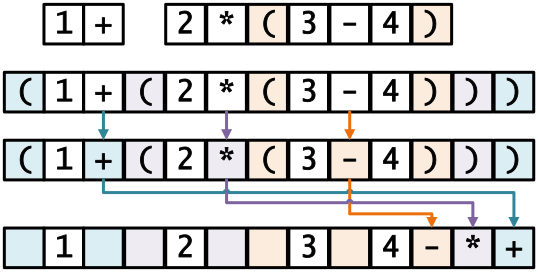
\includegraphics[width=\linewidth]{figures/sta3.pdf}
  \caption{中缀表达式转换为后缀表达式}
  \label{fig:sta3}
\end{figure}


如果要得到前缀表达式,类似地,只需要删掉右括号,将左括号替换为$c$即可。前缀表达式的运算符位于入栈的位置上,而后缀表达式的运算符位于出栈的位置上,这都是非常自然的;反而,我们熟悉的中缀表达式,运算符的位置是不自然的。所以,为了计算中缀表达式,可以先将它转换为前缀表达式或后缀表达式。此处以后缀表达式为例,您可以自行完成前缀表达式的情况。

在手工方法中,操作数仍然在它原本的位置上,而运算符则被移动到了它出栈的位置(必定后于运算符出现的位置)。因此,我们可以对中缀表达式从前到后扫描,当扫描到操作数的时候将其直接加入后缀表达式,而当扫描到运算符的时候将其入栈,在运算符出栈的时候,再将它加入到后缀表达式中。
但是,
当在计算机中处理中缀表达式的时候,并不是每一个运算符都有对应的一对括号,因此,我们需要配合运算符的优先级进行处理。

% 下面,首先从表达式$E$的结构出发进行分析,您可以看到这个思路继承了合法括号序列的分析思想。设$E$的后缀表达式为$\hat{E}$。

% \begin{enumerate}
%     \item 当$E$只包含一个操作数时,$\hat{E}=E$。
%     \item 当$E=(S)$时,$\hat{E} = \hat{S}$。
%     \item 当$E=(S)\ c\ (T)$(其中$c$是运算符)时,$\hat{E} $
% \end{enumerate}

我们的目标是寻找每个运算符应当在哪个位置出栈。我们考虑不为左右括号的运算符$c$,因为左右括号不会被加入到后缀表达式中。考虑表达式$(\ A\ c\ B\ )$,其中,左右的一对括号是$c$对应的括号,$A$和$B$都是表达式。

\begin{enumerate}
    \item 如果这对括号实际存在,那么我们分析表达式$B$的情况。如果$B$是操作数或者被一对括号包裹,则它确实参与了$c$的运算。如果$B$是其他情况,则可以设$B$为$B_1\ c_1\ B_2$,其中$c_1$是$B$在最后一步进行的运算,$B_1$和$B_2$都是表达式。那么,只有$c$的优先级\textit{小于}$c_1$时,$B$作为整体才会参与$c$的运算。否则,在$A\ c\ B_1\ c_1\ B_2$中,会先计算$A\ c\ B_1$,$c$对应的括号应当不包括$\ c_1\ B_2$这一段。
    \item 反过来,如果这对括号实际不存在,那么我们需要定位到它的位置。根据上面的分析可以知道,我们从$c$向后可以继续扫描,直到扫描到优先级\textit{不大于}$c$的运算符$c_1$为止(不包括括号里的运算符)。$c$对应的括号应当出现在$c_1$之前;所以在扫描到$c_1$的时候将$c$出栈。由于我们在上一节中,在表达式两端添加了一堆括号,所以不需要特别判断扫描到末尾的情况(因为末尾一定有实际存在的括号)。
\end{enumerate}

\textit{如果存在右结合运算符,则不等号的严格性会发生变化,(1)中的\textit{小于}应当改为\textit{不大于};(2)中的\textit{不大于}应当改为\textit{小于}。本书实现的运算符中不包含右结合运算符,因此不考虑这个问题;本书的示例代码允许扩展到右结合运算符中,您可以自己尝试将运算符实现为右结合的形式。}

综上所述,我们可以得到这样的算法框架:
\begin{enumerate}
    \item 当扫描到操作数时,直接加入后缀表达式。
    \item 当扫描到非括号的运算符$c$时,首先将栈内优先级不小于$c$的运算符依次弹出并加入后缀表达式,然后将$c$入栈。
\end{enumerate}

现在考虑括号的情况。我们会发现,左括号作为运算符,很难确定它的优先级。一方面,当扫描到左括号的时候,它应当具有最高的优先级,左括号内部永远应当先于当前的栈顶运算符进行计算。另一方面,当左括号在栈内时,它应当具有(除了右括号外)最低的优先级,因为必须计算完括号才能脱括号,所以在找到其对应的右括号之前,任何运算符都不应该让左括号出栈。

这就意味着我们不能用单一的\textit{优先级}来描述运算符,而是需要将其拆分为栈内优先级和栈外优先级。当我们扫描到运算符$c$时,将栈顶的栈内优先级,和$c$的栈外优先级进行比较。如果栈顶的栈内优先级不小于$c$栈外优先级,则将栈顶弹出。左括号出栈后不进入后缀表达式,右括号则不必入栈,因为右括号对应的栈操作是$\land$,扫描到右括号的时候恰好会弹出它对应的左括号。

除了左括号外,其他运算符的栈内和栈外优先级相同;右括号的栈内优先级和栈外优先级都是最低。左括号具有最高的栈外优先级,以及除右括号之外最低的栈内优先级。因此,左括号入栈必定不会引起其他运算符出栈(括号内总是先于括号外计算),且仅当扫描到右括号的时候左括号可以出栈。

\textit{如果您想要同时实现左结合和右结合运算,可以对栈内和栈外的优先级做进一步细化的区分。}在只考虑左结合运算的情况下,两个运算符的比较函数如下。

\begin{lstlisting}
inline static const std::unordered_map<char, int> priority_left {
    {'(', 0}, {')', 0}, {'^', 3}, {'!', 4},
    {'+', 1}, {'-', 1}, {'*', 2}, {'/', 2}, {'%', 2}
};
inline static const std::unordered_map<char, int> priority_right {
    {'(', 6}, {')', 0}, {'^', 3}, {'!', 4},
    {'+', 1}, {'-', 1}, {'*', 2}, {'/', 2}, {'%', 2}
};
bool prior(char next) const override {
    if (isOperator()) {
        auto prior_left { priority_left.find(getOperator()) };
        auto prior_right { priority_right.find(next) };
        if (prior_left != priority_left.end() && prior_right != priority_right.end()) {
            return prior_left->second > prior_right->second;
        }
    }
    return false;
}
\end{lstlisting}

上面虽然进行了很多分析,但目的只是为了让您更好地理解我们为什么要这样设计算法。算法的实际实现非常简单,如下所示。\textit{如果您想要实现前缀表达式,需要改为从后向前扫描,感兴趣的话可以自己完成。}

\begin{lstlisting}
void infix2suffix() {
    Stack<ExpressionElement> S;
    Expression suffix;
    for (auto& e : *this) {
        if (e.isOperand()) {
            suffix.push_back(std::move(e));
        } else {
            while (!S.empty() && S.top().prior(e.getOperator())) {
                if (auto op { S.pop() }; op != '(') {
                    suffix.push_back(std::move(op));
                } else {
                    break;
                }
            }
            if (e != ')') {
                S.push(std::move(e));
            }
        }
    }
    *this = std::move(suffix);
}
\end{lstlisting}

\subsection{后缀表达式转换为中缀表达式}

现在考虑上述问题的反问题:如何从后缀表达式转换为中缀表达式?

下面从信息的角度分析,“中缀转后缀”和“后缀转中缀”有什么不同。
注意到,中缀表达式是由“语义元素”(操作数和非括号的运算符)以及“括号序列”共同组成的。“语义元素”是参与运算的元素,对应了入、出栈过程中操作的数据;而“括号序列”是进行运算的次序,对应了入、出栈过程中的操作序列。所以知道中缀表达式,也就知道了操作序列的每一步入、出栈了什么元素,从而得到入栈序列(前缀表达式)和出栈序列(后缀表达式)。从信息的角度看,中缀表达式中包含的信息,包括了前缀表达式和后缀表达式所需的信息。

但是,后缀表达式仅仅是由“语义元素”组成的,它本身只是一个出栈序列。从前面的小节中您已经知道,给定出栈序列而不给定操作序列,则有$\mathrm{Catalan}(n)$种可能的入栈序列。所以,如果仅仅依赖后缀表达式的\textit{文本},而不借助其他先验信息,那么从后缀表达式反推中缀(前缀)表达式是不可能的、是缺少信息的。要能够实现后缀表达式到中缀表达式的转换,必须要知道\textit{文本}以外的额外信息。

这个先验的额外信息就是:\textit{每个运算符需要的操作数数量}。
在常见的运算符中,加、减、乘、除、乘方,操作数数量都是2;阶乘的操作数数量是1。
需要特别注意的是,当“减号”和“负号”都被作为运算符处理,且采用同一符号$-$时,它的操作数数量是不确定的,这一不确定性会导致后缀表达式出现歧义。中缀表达式可以通过判断$-$之前是否为操作数来进行区分,而后缀表达式无法进行区分。
比如:对于后缀表达式$1\ 2\ -\ 3\ -\ -$,它的三个$-$中有一个代表负号,另外两个代表减号。因此,这个后缀表达式可能对应3种不同的中缀表达式:$1-((-2)-3)$、$(1-2)-(-3)$和$-((1-2)-3)$。
前面几节我们处理中缀表达式的时候,在解析阶段就已经将减号和负号进行了分离。负号被认为是操作数的一部分,而所有出现在表达式中的运算符$-$都是减号;在后缀表达式的处理中我们也将延续这一约定以避免上述歧义。

下面解释,这个先验的额外信息是如何帮助后缀表达式转换成中缀表达式的。\textit{这一部分的内容如果不感兴趣可以略过。}

假设某个运算符$c$的操作数数量是2。在补全了所有括号的中缀表达式中,这个操作数出现在$((A)\ c\ (B))$这个片段里,其中$A$和$B$都是中缀表达式。按照上一节的方法,这个片段化为后缀表达式是$A'\ B'\ c$,其中$A'$和$B'$是$A$和$B$对应的后缀表达式。于是得到:

\begin{theorem}\label{th:后缀表达式1}
对于后缀表达式$E$中的每个运算符$c$,都存在$E$中的一个连续的子序列$E_0$,$E_0$是以$c$结尾的后缀表达式。
\end{theorem}

在之前讨论一般的出栈序列的时候,$A'$和$B'$的划分是任意的,所以会得到卡特兰数的递归方程。但在讨论后缀表达式的时候,需要受到\textit{操作数数量}的限制,因此$A'$和$B'$的划分不是任意的。事实上,只有一种划分是合法的。

我们知道,后缀表达式的开头必定是操作数,末尾必定是运算符。对于语义元素组成的序列$C=(c_1,c_2,\dots,c_n)$,定义:
$$
f(c_i)=\begin{cases}
1,&c_i\mathrm{\ is\ operand},\\
1-\mathrm{Cnt}(c_i),&c_i\mathrm{\ is\ operator\ with\ Cnt\ operands}
\end{cases}
$$

\begin{theorem}\label{th:后缀表达式2}
令$f(C)=\sum f(c_i)$,则对于合法的后缀表达式$E$,$f(E)=1$。
\end{theorem}

\begin{proof}
使用数学归纳法,对$E$中含有的运算符数量归纳。

\begin{enumerate}
    \item 对于单个操作数,$f(E)=1$。
    \item 对于以$k$元运算符结尾的表达式,设$E$为$A_1\ A_2\ \dots \ A_k\ c$,其中$A_i$是后缀表达式。从而$f(E) = \sum f(A_i) + f(c) = k + (1-k) = 1$。
\end{enumerate}
\end{proof}
\begin{theorem}\label{th:后缀表达式3}
对于合法后缀表达式$E$的任意前缀$E_j=(e_1,e_2,\dots,e_j),j\le n$,始终有$f(E_j)\ge 1$。
\end{theorem}

\begin{proof}
使用数学归纳法,对$j$归纳。

\begin{enumerate}
    \item 由于$e_1$是操作数,所以$f(E_1)=1$。
    \item 如果$e_j$是操作数,则$f(E_j)=f(E_{j-1})+1\ge 1+1>1$。
    \item 如果$e_j$是运算符,根据定理\ref{th:后缀表达式1},必定存在某个$(e_t,e_{t+1},\dots,e_j),1\le t<j$是以$e_j$结尾的后缀表达式。那么根据定理\ref{th:后缀表达式2},$f(e_t,e_{t+1},\dots,e_j)=1$,从而$f(E_j)=f(E_{t-1}) + f(e_t,e_{t+1},\dots,e_j)\ge f(e_t,e_{t+1},\dots,e_j)=1$。
\end{enumerate}
\end{proof}

\begin{theorem}
    对于以$k$元运算符$c$结尾的后缀表达式$E$,只有唯一的合法划分方式使$E$被划分为$A_1\ A_2\ \dots\ A_k\ c$。
\end{theorem}

\begin{proof}
使用反证法证明。

    如果有不止一种合法的划分方式,设两种划分方式中$(A_1,A_2,\dots,A_k)$序号最大的一个不同的项是$A_j$和$A_j'$。不妨设$A_j$的长度大于$A_j'$,那么$A_j$则可以被拆分为两段$P\ A_j'$。因为$A_j$和$A_j'$都是合法的后缀表达式,所以由定理\ref{th:后缀表达式2},$f(P) = f(A_j) - f(A_j') = 1-1=0$。但是$P$是$A_j$的前缀,根据定理\ref{th:后缀表达式3}应有$f(P)\ge 1$,矛盾。
\end{proof}

因此,递归地进行唯一合法的划分,就可以得到最终的中缀表达式。\textit{类似地,您可以得到前缀表达式转换为中缀表达式的手段。}

需要说明的是,上面的转换方式并不实用,笔者在此处也没有给出相应的示例代码,仅仅从理论的角度进行介绍。
实际转换的时候,通常利用\textbf{表达式树}作为中介进行转换,表达式树的内容将会在后面的章节介绍。在本章介绍表达式,是希望您在思维中巩固“栈”和“表达式”之间的联系。

\subsection{后缀表达式转换为前缀表达式}
在上一小节中使用了一个$f(\cdot)$函数用来辅助证明,这个函数并不是凭空产生的,而是另一个栈的产物。我们采用下面的方法构造一个操作序列。

\begin{enumerate}
    \item 将后缀表达式中的操作数$i$,用$\lor(i)$替代。
    \item 将后缀表达式中的运算符$c$,用$\land ^k \lor(c)$替代,其中$\land^k$表示$k$个连续的$\land$,$k$是这个运算符的运算所需操作数数量。
    \item 在整个序列的结尾处增加一个$\land$。
\end{enumerate}


根据上一小节的定理\ref{th:后缀表达式2}和定理\ref{th:后缀表达式3},我们可以确定,这样得到的操作序列是合法的。

我们发现,在这个操作序列中,对应的\textit{入栈序列恰好是后缀表达式}。自然地,我们想到要分析它的出栈序列。仍然以前面的$1\ 2\ 3\ 4\ -\ *\ +$作为例子,它对应$\lor(1)\ \lor(2)\ \lor(3)\ \lor(4)\ \land\ \land\ \lor(-)\ \land\ \land\ \lor(*)\ \land\ \land\ \lor(+)\ \land$,从而可以得到出栈序列是$4\ 3\ -\ 2\ *\ 1\ +$。这恰好是\textit{倒序的前缀表达式}。\textit{对于一般情形,您可以用递归(归纳)的方法证明这个结论。对偶地,您也可以得到前缀表达式转换成后缀表达式的手段。}

\subsection{后缀表达式的计算}

后缀表达式的计算是考试中的传统题型之一。要计算后缀表达式,只需要对上一小节中的操作序列作出一点点修改。

\begin{enumerate}
    \item 将后缀表达式中的操作数$i$,用$\lor(i)$替代。
    \item 将后缀表达式中的运算符$c$,用$\land ^k \lor(r)$替代,其中$\land^k$表示$k$个连续的$\land$,$k$是这个运算符的运算所需操作数数量。$r$是\textit{本次运算的结果}。设第$i$个$\land$出栈的数为$A_i$,则$r=c(A_1,A_2,\dots,A_k)$。
    \item 在整个序列的结尾处增加一个$\land$。这次出栈的数就是后缀表达式的计算结果。
\end{enumerate}

这个算法的正确性也可以递归证明。您可以自己实现这一算法的代码,下面展示了一个示例。

\begin{lstlisting}
int calSuffix() const {
    Stack<int> S;
    for (auto& e : *this) {
        if (e.isOperand()) {
            S.push(e.getOperand());
        } else {
            auto [l, r] { e.operandPosition() };
            int rhs { r ? S.pop() : 0 };
            int lhs { l ? S.pop() : 0 };
            S.push(e.apply(lhs, rhs));
        }
    }
    return S.pop();
}
\end{lstlisting}

考试中实际出现的后缀表达式计算题目,可以使用上述算法手工计算。
不过和之前一样,笔者推荐使用表达式树而不是栈进行计算。
诚然,表达式树的做法比栈要复杂一些;但表达式树的方法更加清晰,更加适合答题结束后的检查,更加不容易出错。

知道后缀表达式如何计算之后,由于之前已经介绍过各种表达式之间互相转换的方法,所以您也就能够写出计算前缀表达式和中缀表达式的算法了。

\subsection{实验:中缀表达式的计算}
\label{sta:中缀表达式的计算}
在这个实验中将实现中缀表达式的计算,从而实现一个类似计算器的功能。代码可以在\textit{Expression.cpp}中找到。

\begin{lstlisting}
class CalExpr : public Algorithm<int, const string&> {};
\end{lstlisting}

根据前面的结论,我们可以先将中缀表达式转换为后缀表达式,再使用后缀表达式计算。

\begin{lstlisting}
int operator()(const string& expr) override {
    Expression e { expr };
    e.infix2suffix();
    return e.calSuffix();
}
\end{lstlisting}

因为无论是中缀转后缀,还是后缀求值,都是从左到右依次进行,所以我们也可以将中缀转后缀和后缀求值的过程合并在一起。此时,因为运算符的优先级只能和运算符相比,所以需要使用两个栈,将运算符和表达式拆开。如下所示。

\begin{lstlisting}
int calInfix() const {
    Stack<int> Sr;
    Stack<ExpressionElement> So;
    for (auto& e : *this) {
        if (e.isOperand()) {
            Sr.push(e.getOperand());
        } else {
            while (!So.empty() && So.top().prior(e.getOperator())) {
                if (auto op { So.pop() }; op != '(') {
                    auto [l, r] { op.operandPosition() };
                    int rhs { r ? Sr.pop() : 0 };
                    int lhs { l ? Sr.pop() : 0 };
                    Sr.push(op.apply(lhs, rhs));
                } else {
                    break;
                }
            }
            if (e != ')') {
                So.push(e);
            }
        }
    }
    return Sr.pop();
}
\end{lstlisting}

我们的实验中提供了一些简单的例子来测试它的正确性,并使用大量的1相加来对算法的性能进行简单的测定。直接计算的常数会比通过后缀表达式间接计算低一些,但是差距非常小,几乎可以忽略不计。

如果您使用了合取方法来定义表达式中的元素,则上面的算法可以得到大幅度简化:因为表达式里的每个元素都是运算符,而操作数是附带在前方最近的运算符上的。推荐您进行这样的尝试。此外,引入$k$元运算符也是一个有趣的修改方向。您可能会发现,\lstinline{operandPosition}中包含的位置信息并没有实际的作用,事实上我们只需要知道一个运算符具有多少个参数。我们修改这个方法,并将\lstinline{apply}实现为接受向量(而不是数对)的方法,即可兼容任意元运算符。这里需要使用向量而不是可变参数包的原因是,我们无法在编译期知道参数列表的长度。

\section{栈与递归}

栈和递归的关系非常紧密,因为调用递归函数本质上相当于使用了系统栈。具体的原理参见《操作系统》。系统栈的空间是有限的,如果递归层次过多,就会发生栈溢出(stack overflow)错误。为了避免这种情况发生,我们可以通过手写栈将递归改写为迭代形式。本节将介绍使用栈消除递归的方法。

\subsection{实验:消除尾递归的扩展形式*}
\label{sta:消除扩展尾递归}
在\ref{vec:消除简单尾递归}节,我们介绍了消除尾递归的方法。尾递归因为每个递归实例只会在尾部调用一次自身,所以不需要使用栈。在这一小节,我们将介绍一种尾递归的扩展形式:每个递归实例会在尾部调用不止一次自身。这样的递归函数通常没有返回值。

在这一节,我们制造一个没有返回值的场景来对这种情况进行分析。给定$w$,求$w$个数位均为1、2、3或4的$w$位十进制数的数量。当然,我们知道答案是$4^w$,不过我们希望将所有符合条件的数枚举一遍,放入一个向量中,最后再返回向量的规模。代码可以在\textit{Generate4.cpp}中找到。

\begin{lstlisting}
class Generate4 : public Algorithm<size_t(size_t)> {
protected:
    Vector<size_t> V;
};
\end{lstlisting}

我们可以写出这样的递归算法,对所有符合条件的数进行枚举。
\begin{lstlisting}
class Generate4Solver : public Algorithm<void(Vector<size_t>&, size_t)> {
protected:
    size_t minn, maxn;
public:
    Generate4Solver() = default;
    Generate4Solver(size_t w) : minn(Power {}(10, w - 1)), maxn(Power {}(10, w) - 1) {}
};

class Generate4RecursiveSolver : public Generate4Solver {
public:
    void operator()(Vector<size_t>& V, size_t n) override {
        if (minn <= n && n <= maxn) {
            V.push_back(n);
        } else {
            for (size_t i : {1, 2, 3, 4}) {
                (*this)(V, n * 10 + i);
            }
        }
    }
};
\end{lstlisting}

从上述算法中,我们可以很快提取到一些关键信息。
\begin{enumerate}
    \item 递归边界:$n\in \left[10^{w-1},10^w\right)$。
    \item 递归边界上的返回:将$n$加入向量。
    \item 非递归边界时的调用:$10n+j$,其中$j=1,2,3,4$。
\end{enumerate}

类似于只调用一次自身的尾递归,我们可以拟造出递归形式的模板。和尾递归的区别主要有两个:(1)没有返回值;(2)非递归边界时的调用返回包含多组参数的向量。

\begin{lstlisting}
void operator()(Args... args) override {
    if ((*pred)(args...)) {
        (*bound)(args...);
    } else {
        for (auto&& nextArgs : (*next)(args...)) {
            apply(*this, nextArgs);
        }
    }
}
\end{lstlisting}

在我们的例子中,每个非边界的递归实例会调用4次自身(尾递归)。记递归函数为$f$,那么首先调用$f(10n+1)$,完成它的所有递归实例之后再进入$f(10n+2)$。这个过程类似于我们定义了一个4元运算符$c$,在计算后缀表达式$(A_1)\ (A_2)\ (A_3)\ (A_4)\ c$,其中$A_j$表示$f(10n+j)$。我们可以仿照后缀表达式的计算,在$A_1$全部计算完成之后再让$A_2$开始入栈;但因为我们是从上到下递归计算的,所以我们可以一并将$A_4\ A_3\ A_2\ A_1$\textit{倒序}入栈,这样,$A_1$会成为栈顶,$A_1$全部计算完成之后$A_2$成为栈顶,以此类推。下面是一个利用栈的迭代实现的模板,其中特别需要注意采用了倒序遍历。

\begin{lstlisting}
void operator()(Args... args) override {
    Stack<tuple<Args...>> S { { args... } };
    while (!S.empty()) {
        tie(args...) = S.pop();
        if ((*pred)(args...)) {
            (*bound)(args...);
        } else {
            for (auto&& nextArgs : (*next)(args...) | views::reverse) {
                S.push(move(nextArgs));
            }
        }
    }
}
\end{lstlisting}

套用模板,可以得到Generate4问题的迭代版本。它和前面的递归版本等价。

\begin{lstlisting}
void operator()(Vector<size_t>& V, size_t n) override {
    Stack<size_t> S { n };
    while (!S.empty()) {
        n = S.pop();
        if (minn <= n && n <= maxn) {
            V.push_back(n);
        } else {
            for (size_t i : {4, 3, 2, 1}) {
                S.push(n * 10 + i);
            }
        }
    }
}
\end{lstlisting}

类似于尾递归的情况,使用模板总是比不使用慢。但和尾递归的情况不同,采用栈进行迭代反而会慢于直接递归。同时,采用栈进行迭代也不会降低算法的空间复杂度,因此它通常只作为一种避免栈溢出系统错误的手段,在平时书写代码的时候并不实用。递归的高速的得益于编译器的优化;这告诉我们挑战编译器的能力边界,对绝大多数编程人员来说都是极具浪漫主义色彩的冒险行为。

\subsection{实验:计算组合数*}
\label{sta:计算组合数}
对上一节介绍的尾递归扩展形式稍作改动,可以用来计算一些有返回值的递归函数。这些函数在计算完每个递归调用的结果之后,对这些结果进行一个简单的处理,然后返回。本节以计算组合数的问题作为例子,代码可以在\textit{Combine.cpp}中找到。

众所周知,组合数满足递归公式:
$$
\mathrm{C}_n^m = \begin{cases}
    1,&m=0\mathrm{\ or\ }m=n,\\
    \mathrm{C}_{n-1}^{m-1}+\mathrm{C}_{n-1}^m,&\mathrm{otherwise}
\end{cases}
$$

基于这个公式,可以设计下面的算法。

\begin{lstlisting}
// CombineRecursive1
int operator()(int n, int m) override {
    if (m == 0 || m == n)
        return 1;
    return (*this)(n - 1, m - 1) + (*this)(n - 1, m);
}
\end{lstlisting}

它和上一节介绍的尾递归扩展形式的不同在于,在递归调用两个实例之后,还进行了一次加法。看起来由于加法的存在,这个算法似乎不是尾递归;但是,我们可以通过将加法“吸收”到递归函数内部,将它改写成上一节的形式。如下所示。

\begin{lstlisting}
class CombineRecursive2 : public CombineProblem {
    int sum { 0 };
    void combine(int n, int m) {
        if (m == 0 || m == n) {
            ++sum;
        } else {
            combine(n - 1, m - 1);
            combine(n - 1, m);
        }
    }
public:
    int operator()(int n, int m) override {
        sum = 0;
        combine(n, m);
        return sum;
    }
};
\end{lstlisting}

接着,我们可以使用上一节的模板,将其改写为使用栈进行迭代的形式。

\begin{lstlisting}
int operator()(int n, int m) override {
    int sum { 0 };
    Stack<pair<int, int>> S { {n, m} };
    while (!S.empty()) {
        auto [n, m] { S.pop() };
        if (m == 0 || m == n) {
            ++sum;
        } else {
            S.push({ n - 1, m - 1 });
            S.push({ n - 1, m });
        }
    }
    return sum;
}
\end{lstlisting}

需要指出的是,这个方法是极其低效的,因为$\mathrm{sum}$只能不断加一,所以该方法的时间复杂度高达$\Theta\left(\mathrm{C}_n^m\right)$。其中,使用栈的方法将比递归更加低效。为了提高时间效率,我们可以利用之前介绍过的\textit{不必要工作}对算法的过程进行检查。我们可以发现,在这个计算过程中包含了大量的\textit{重复工作},比如,$\mathrm{C}_n^m=\mathrm{C}_{n-1}^{m-1}+\mathrm{C}_{n-1}^m=\mathrm{C}_{n-2}^{m-2}+2\mathrm{C}_{n-2}^{m-1}+\mathrm{C}_{n-2}^m$,因而$\mathrm{C}_{n-2}^{m-1}$被计算了2次。为了解决这个问题,我们可以利用\textbf{记忆化搜索}(memory search)的技术,将我们已经计算过的结果储存起来,如下所示。

\begin{lstlisting}
class CombineMemorySearch : public CombineProblem {
    vector<vector<int>> C;
    void initialize(size_t n) {
        C.resize(n + 1);
        for (size_t i = 0; i <= n; ++i) {
            C[i].resize(i + 1, 0);
            C[i][0] = C[i][i] = 1;
        }
    }
public:
    int operator()(int n, int m) override {
        if (n >= C.size())
            initialize(n);
        if (C[n][m] == 0) {
            C[n][m] = (*this)(n - 1, m - 1) + (*this)(n - 1, m);
        }
        return C[n][m];
    }
};
\end{lstlisting}

上述算法的空间复杂度为$\Theta(n^2)$;在不考虑初始化的情况下,最坏时间复杂度为$\Theta(m(n-m))$。它的好处是在计算$\mathrm{C}_n^m$的时候可以得到很多中间结果,当我们反复调用它的时候,这些储存下来的中间结果可以得到复用,从而降低了分摊的时间消耗。如果我们只需要计算$\mathrm{C}_n^m$这一个数,有更快的计算方法,那就是直接利用$\mathrm{C}_n^m=\frac{(n+m)!}{n!m!}$这个公式:这个公式一共只需要进行$\Theta(m)$次计算(上下的$n!$可以被约去),从而我们可以做到$O(1)$的空间复杂度和$\Theta(m)$的时间复杂度。\textit{您可以自己完成这个算法。}

测试表明,Recursive2的效率会明显高于Recursive1,这说明了尾递归在编译器优化上的优势。当我们有机会使用尾递归的时候,应当尽可能使用尾递归。

\subsection{实验:消除一般的递归*}

在前面两节中,我们从尾递归过渡到了它的扩展形式,允许函数进行多次递归调用。
对于一般的递归而言,这多次递归调用不一定出现在尾部,递归调用之间可以穿插其他代码。我们可以将一般的递归概括为下面的形式。

\begin{lstlisting}
R operator()(Args... args) override {
    if ((*pred)(args...)) {
        return (*bound)(args...);
    } else {
        vector<R> V {};
        while ((*hasnext)(V, args...)) {
            V.push_back(apply(*this, (*next)(V, args...)));
        }
        return (*finalize)(V, args...);
    }
}
\end{lstlisting}

由于递归调用依赖于此前的递归调用结果,所以在这种情况下,我们没法一次性地将所有递归调用的参数入栈,需要将用来存储已有递归调用结果的向量$V$也缓存在栈内。

\begin{lstlisting}
R operator()(Args... args) override {
    vector<R> V {};
    Stack<tuple<vector<R>, Args...>> S { { {}, args... }, { {}, args... } };
    while (S.size() > 1) {
        tie(V, args...) = S.top();
        optional<R> r {};
        if ((*pred)(args...)) {
            r = (*bound)(args...);
        } else if ((*hasnext)(V, args...)) {
            tie(args...) = (*next)(V, args...);
            S.push({ {}, args... });
        } else {
            r = (*finalize)(V, args...);
        }
        if (r.has_value()) {
            S.pop();
            get<0>(S.top()).push_back(r.value());
        }
    }
    return get<0>(S.top())[0];
}
\end{lstlisting}

这里在栈中预先存放了一个空向量,用来存储最终返回的值。上述形式肉眼可见地低效,仅仅作为考试中需要改写为迭代形式而没有找到合适方法时,保底的通用解法。您可以在\textit{Generate4Sum.cpp}中看到一个使用例子。

\section{栈的扩展}

\subsection{共享栈}

当我们使用顺序栈的时候,我们为栈申请了一片连续内存作为存储空间。注意到,我们的栈只使用了前半部分的空间,而没有使用后半部分的空间。有一种高效利用空间的方法称为\textbf{共享栈}(shared stack),它由两个共享同一片连续内存的栈组成。其中一个栈使用前半部分,以秩为0的元素为栈底,以秩最大的元素为栈顶;另一个栈使用后半部分,以秩为$n-1$的元素为栈底,以秩最小的元素为栈顶。两个栈的栈顶“相向而行”。由于现在往往不需要如此精打细算空间消耗,现在已经很少看到这个数据结构,邓书也不介绍它。您可以将此作为栈的一个练习自己实现,并使用\textit{SharedStackTest.cpp}测试。

我们使用向量$V$(而不是数组)作为实现共享栈的基础,以提供变长特性。使用两个变量\lstinline{topf}和\lstinline{topb}分别表示前向栈(栈顶向秩大的方向移动)和后向栈(栈顶向秩小的方向移动)的栈顶位置。在我们的设计中,这两个变量均代表“下一个”的值,比如前向栈的栈顶元素是$V[2]$时,\lstinline{topf}的值是3,后向栈的栈顶元素是$V[2]$时,\lstinline{topb}的值是1。您也可以记录栈顶元素本身的秩。

接下来,我们利用类的嵌套,具体构造两个栈。这里展示了后向栈的设计,前向栈与其大体相同。

\begin{lstlisting}
class BackwardStack : public AbstractStack<T> {
    SharedStack& S;
public:
    BackwardStack(SharedStack& s) : S(s) {}
    void push(const T& e) override {
        S.V[S.m_topb--] = e;
    }
    T& top() override {
        return S.V[S.m_topb + 1];
    }
    T pop() override {
        return std::move(S.V[++S.m_topb]);
    }
    size_t size() const override {
        return S.V.size() - 1 - S.m_topb;
    }
};
\end{lstlisting}

唯一需要注意的是,在进行入栈操作的时候,除了上面的基本操作,还需要进行一次共享栈是否已满(是否已经接触到另一个栈的栈顶)的判定。如果共享栈已满,则需要进行扩容。我们可以使用向量本身的扩容,然后将后向栈移动到向量尾部的位置。

\begin{lstlisting}
void expand() {
    size_t oldsize { V.size() };
    V.resize(std::max(V.capacity() + 1, V.capacity() * 2));
    std::move_backward(V.begin() + m_topb + 1, V.begin() + oldsize, V.end());
    m_topb += V.size() - oldsize;
}
\end{lstlisting}

\textit{为了和您自己实现的向量类兼容,此处没有对向量自身的扩容策略进行萃取,而是采用了固定的2倍扩容策略,您可以将其改为自己的扩容策略,或者改为萃取的形式。}

经典的向量中,空闲的元素位于内存的尾部,而共享栈中,空闲的元素位于内存的中部,因此不适用向量本身的规模机制。您可以认为这里的两个指针\lstinline{topf}和\lstinline{topb}实现了和向量中的\lstinline{size}同样的内存管理功能。

\subsection{最小栈*}
\label{sta:最小栈}
栈对于用户可以访问的位置做出了很强的限制,有时我们希望略微放开这些限制,使得用户可以访问到一些更多的信息。\textbf{最小栈}(minimum stack)是其中的一个典型的例子。在最小栈中除了栈本身所支持的三种基本操作之外,还支持\lstinline{min}操作,返回当前栈内元素的最小值。要求在栈的三种基本操作的分摊复杂度保持$O(1)$的前提下,新增的\lstinline{min}操作的分摊复杂度也为$O(1)$。这里假定比较两个元素的操作时间复杂度为$O(1)$。您自己实现的最小栈可以使用\textit{MinStackTest.cpp}测试。

一个基本的思想是维护一个变量$m$来存储栈中的最小值。
当插入的元素$e<m$的时候更新$m$没有问题,但当删除的元素$e=m$的时候,我们既不知道这个$e$是否是当前栈中唯一的最小值$m$,又不知道当唯一最小值被删除之后,新的最小值是多少。这就导致如果我们进行连续的删除操作,则需要反复地遍历整个栈来寻找新的最小值。这在两个方面不能达到我们的要求。

\begin{enumerate}
    \item 时间复杂度上会存在问题。弹出元素的时候,时间复杂度高达$\Theta(n)$,而无法满足我们需求的$O(1)$。
    \item 栈的性质上会存在问题。我们不应当访问栈顶以外的其他元素,即使在栈的实现内部也是如此。
\end{enumerate}

为了在弹出元素的时候,能够立刻找到新的最小值,我们想到用空间换时间的方法。我们定义一个辅助线性表$S_m$,规定$S_m[k] = \min (S[0],S[1],\dots,S[k])$。因为栈$S$只能在栈顶进行操作,而$S_m[k] = \min(S_m[k-1],S[k])$,所以$S_m$也只会在尾部进行操作,它同样是一个栈。

\begin{lstlisting}
template <typename T>
class MinStack : public Stack<T> {
    Stack<T> minStack;
public:
    void push(const T& e) override {
        Stack<T>::push(e);
        if (minStack.empty()) {
            minStack.push(this->top());
        } else if (auto t { minStack.top() }; t < this->top()) {
            minStack.push(t);
        } else {
            minStack.push(this->top());
        }
    }
    T pop() override {
        minStack.pop();
        return Stack<T>::pop();
    }
    const T& min() const {
        return minStack.top();
    }
};
\end{lstlisting}

上面的实现方式需要$\Theta(n)$的额外空间。
我们可以发现,在辅助栈中存在大量重复的元素。比如,在栈$S=[3, 4, 5, 1, 2\rangle $时,辅助栈$S_m = [3, 3, 3, 1, 1\rangle$,其中3被重复了3次,1被重复了2次。因此,直觉上看存在空间复杂度并非最优的可能性。
为了判断是否已经取得了最优的空间复杂度,我们需要对辅助栈进行分析。
考虑一个略简单的模型,即栈内的元素互不相等的情况:设栈中的元素为$1,2,\dots,n$。我们对辅助栈和栈操作序列建立一个一一对应。

\begin{enumerate}
    \item 补充定义$S_m[-1]=n+1$。对于$S[j]$,如果$S[j]\ne S[j-1]$,则将$S[j]$替换为$\lor ^{k}\land$,其中$k = S[j-1] - S[j]$。
    \item 如果$S[j] = S[j-1]$,则将$S[j]$替换为$\land$。
\end{enumerate}

\textit{请您自己证明上面的这个映射得到的操作序列是合法的。}因此,辅助栈的所有可能情况数量为$\mathrm{Catalan}(n)$。从信息论的角度看,我们至少需要$\log\left(\mathrm{Catalan}(n)\right)$的空间才能表示这些情况。又因为
$$
\log\left(\mathrm{Catalan}(n)\right) \sim 2n\log \left(\frac{2n}{e}\right) - 2n \log \left(\frac{n}{e}\right)  \sim 2n
$$

当允许元素相等的时候,情况只会更多,需要的空间也只会更多。
因此,无论采用如何的方式,只要存储了辅助栈,那么在最坏情况下需要的额外空间复杂度总是$\Theta(n)$。

下面将介绍另一种最小栈的实现方法。该方法极具迷惑性,它看起来空间复杂度为$O(1)$,但实际上仍然为$\Theta(n)$。\textit{尚不清楚此类方法是否在考试中被认为是$O(1)$方法。}

根据之前的分析,如果采用辅助栈$S_m$来存储每个前缀的最小值,则需要至少$\Theta(n)$的空间。因此,
如果我们想要降低空间复杂度,就必须抛弃辅助栈的设计。我们观察辅助栈和原栈之间的联系:如果辅助栈在第$k$个位置发生了变化$x\to y$,也就意味着原栈的第$k$个位置插入了$y$,并且$y<x$。现在我们不想要辅助栈,也就是说我们需要借助原栈的信息从$y$还原到$x$。

一个直接的想法是,在原栈的每个位置上存数据对$(x,S[k])$,其中$S[k]$是栈在该位置上的实际元素,$x$则是该位置被弹出之后的新的最小值。采用一个额外变量$y$来维护当前的最小值,当$(x,S[k])$被弹出时,令$y=x$。当然,我们知道这个方法和最小栈实质上完全一样,同样需要$\Theta(n)$的辅助空间。

于是我们想到对这个数据对进行变形,改为存一个映射的象$z=f(x,S[k])$。那么,我们需要在已知$y$和$z$的情况下,能够还原出$x$和$S[k]$。如果仅凭$z$还原,就是上面的数据对思路,$z$的信息量是$x$和$S[k]$的和,需要$\Theta(n)$的辅助空间。所以我们会想到,$y$也能提供一部分信息,$z$中需要存储的信息量可以下降。于是,我们可以把这个映射表述为$(y,z) = \mathbf{F}(x, S[k])$,其中$y$的语义是确定的,即$y = \min (x,S[k])$。

直观上看,$\mathbf{F}$输入两个值,输出两个值,那么可以让$x,S[k]$的信息完全被包含在$y,z$中;但事实并非如此。由于$y = \min(x, S[k])$打破了对称性,导致$y$包含的信息量降低了,从而使得$z$需要包含更多的信息量。
假设$x,S[k]$都是某个$m$元集中,等概率随机选取的元素,那么$(x,S[k])$的信息熵为$2\log m$,而$y=\min (x, S[k])$的信息熵为
$$
H(y) = -\sum_{k=1}^{m} \frac{2k-1}{m^2} \log  \frac{2k-1}{m^2} = \log n -\sum _{k=1}^m \frac{2k-1}{m^2}\log \frac{2k-1}{m}
$$
$$
= \log m - \frac{1}{2}\sum _{k=1}^m \frac{2}{m}\cdot \frac{2k-1}{m}\log \frac{2k-1}{m} 
= \log m - \frac{1}{2} \int_0^{2} x\log x \mathrm{d}x + o(1)
$$
$$
= \log m - \left(1 - \frac{1}{2\ln 2}\right) + o(1)
$$

上述计算结果表明,$H(y)$和$\log m$之间存在$\theta = 1 - \frac{1}{2\ln 2}\approx 0.28$的差距,这使得每个$z$需要额外的至少0.28比特来存储这些损失的信息,使用和$S[k]$一样的空间是做不到的。

我们知道$y = \min(x, S[k])$,一个非常简单的想法就是令$z = \max(x, S[k])$。这样,我们通过$(y,z)$就能确定$\{x,S[k]\}$,只是分不清楚哪个是$x$、哪个是$S[k]$。只要增加1个比特(通常称为\textbf{标志位})来指示这一点,就可以实现逆运算$(x,S[k]) = \mathbf{F}^{-1}(y,z)$。

作为举例,如果我们保证栈内的所有元素都非负,就可以让符号位作为标志位,即:
$$
z = \begin{cases}
    S[k],&S[k]\ge x,\\
    -x,&S[k]<x
\end{cases}
$$

此时还原的方法为:
$$
\begin{cases}
    x &= |\min(y,z)|,\\
    S[k] &= \max(y,z)
\end{cases}
$$

在实际软件开发中,带符号整数的比特数通常只能取16、32、64等标准位宽以做到字节对齐;所以通常都允许我们划出一些比特来存储额外的信息。但从本质上来说,这种方法仍然具有$\Theta(n)$的空间开销(每个元素包含了1个标志位)。

您可能会注意到,在前面使用信息论方法说明辅助栈需要的空间时,空间复杂度的常数至少为2;但上述的标志位方法常数为1。这并不是突破了信息论的限制,而是因为辅助栈中的一些信息是包含在原栈里的。比如,在知道原栈的情况下,$S_m = [3,3,3,1,1\rangle$和$S_m = [2,2,2,1,1\rangle$可以以相同的方式表示,因为二者都是3个$S[0]$和2个$S[3]$,这降低了描述辅助栈需要的信息量。上述表示方式的数量,相当于将$n$个元素划分成任意多的段的划分数量,也就是$2^{n-1}$,因此至少需要$\log \left(2^{n-1}\right) = n-1$个比特进行刻画;这正好对应了$z_1,z_2,\dots,z_{n-1}$的标志位。$z_0$的标志位没有包含任何信息,因为只有一个元素的情况下,最小值必然是它本身。

\section{本章小结}
作为适配器的栈本身非常简单,无论采用顺序栈还是链栈进行实现都没有难度。初学者可能会好奇,栈能做到的事情线性表(向量或列表)都能做到,为什么要自己给自己设限制呢?这个问题的答案,和OOP中将一些方法设置为私有的原因是一样的。通过加以限制,我们的目光被聚焦了,更容易抓住解决问题的要点。

栈的操作很简单,
这也就意味着,将其他复杂的问题,比如括号匹配、表达式计算等转化为栈的问题,可以让问题得到大幅的简化。本章的主要学习目标如下。
\begin{enumerate}
    \item 您理解了栈操作序列的性质,在遇到相似性质的场景时可以联想到用栈解决。
    \item 您了解到出栈序列的计数是卡特兰数,在遇到相似的递归方程时可以联想到用栈解决。
    \item 您掌握了利用栈将任意递归改写为迭代的技术。
\end{enumerate}


% \subsection{单调栈}

% 在上一节中使用的辅助栈$S_m$是一个典型的\textbf{单调栈}(monotonous stack)。栈内的元素单调(可以且经常是非严格的单调)的栈称为单调栈。



% \chapter{引用文献的标注}

% 模板支持 BibTeX 和 BibLaTeX 两种方式处理参考文献。
% 下文主要介绍 BibTeX 配合 \pkg{natbib} 宏包的主要使用方法。


% \section{顺序编码制}

% 在顺序编码制下,默认的 \cs{cite} 命令同 \cs{citep} 一样,序号置于方括号中,
% 引文页码会放在括号外。
% 统一处引用的连续序号会自动用短横线连接。

% \thusetup{
%   cite-style = super,
% }
% \begin{tabular}{l@{\quad$\Rightarrow$\quad}l}
%   \verb|\cite{zhangkun1994}|               & \cite{zhangkun1994}               \\
%   \verb|\citet{zhangkun1994}|              & \citet{zhangkun1994}              \\
%   \verb|\citep{zhangkun1994}|              & \citep{zhangkun1994}              \\
%   \verb|\cite[42]{zhangkun1994}|           & \cite[42]{zhangkun1994}           \\
%   \verb|\cite{zhangkun1994,zhukezhen1973}| & \cite{zhangkun1994,zhukezhen1973} \\
% \end{tabular}


% 也可以取消上标格式,将数字序号作为文字的一部分。
% 建议全文统一使用相同的格式。

% \thusetup{
%   cite-style = inline,
% }
% \begin{tabular}{l@{\quad$\Rightarrow$\quad}l}
%   \verb|\cite{zhangkun1994}|               & \cite{zhangkun1994}               \\
%   \verb|\citet{zhangkun1994}|              & \citet{zhangkun1994}              \\
%   \verb|\citep{zhangkun1994}|              & \citep{zhangkun1994}              \\
%   \verb|\cite[42]{zhangkun1994}|           & \cite[42]{zhangkun1994}           \\
%   \verb|\cite{zhangkun1994,zhukezhen1973}| & \cite{zhangkun1994,zhukezhen1973} \\
% \end{tabular}



% \section{著者-出版年制}

% 著者-出版年制下的 \cs{cite} 跟 \cs{citet} 一样。

% \thusetup{
%   cite-style = author-year,
% }
% \begin{tabular}{l@{\space$\Rightarrow$\space}l}
%   \verb|\cite{zhangkun1994}|                & \cite{zhangkun1994}                \\
%   \verb|\citet{zhangkun1994}|               & \citet{zhangkun1994}               \\
%   \verb|\citep{zhangkun1994}|               & \citep{zhangkun1994}               \\
%   \verb|\cite[42]{zhangkun1994}|            & \cite[42]{zhangkun1994}            \\
%   \verb|\citep{zhangkun1994,zhukezhen1973}| & \citep{zhangkun1994,zhukezhen1973} \\
% \end{tabular}

% \vskip 2ex
% \thusetup{
%   cite-style = super,
% }
% 注意,引文参考文献的每条都要在正文中标注
% \cite{zhangkun1994,zhukezhen1973,dupont1974bone,zhengkaiqing1987,%
%   jiangxizhou1980,jianduju1994,merkt1995rotational,mellinger1996laser,%
%   bixon1996dynamics,mahui1995,carlson1981two,taylor1983scanning,%
%   taylor1981study,shimizu1983laser,atkinson1982experimental,%
%   kusch1975perturbations,guangxi1993,huosini1989guwu,wangfuzhi1865songlun,%
%   zhaoyaodong1998xinshidai,biaozhunhua2002tushu,chubanzhuanye2004,%
%   who1970factors,peebles2001probability,baishunong1998zhiwu,%
%   weinstein1974pathogenic,hanjiren1985lun,dizhi1936dizhi,%
%   tushuguan1957tushuguanxue,aaas1883science,fugang2000fengsha,%
%   xiaoyu2001chubanye,oclc2000about,scitor2000project%
% }。
